% ==========================================
% MAIN.TEX - LUXEWAY RESEARCH PAPER
% IEEE Conference Format (IEEEtran)
% ==========================================
\documentclass[conference]{IEEEtran}

% --- Core packages ---
\usepackage[T1]{fontenc}
\usepackage[utf8]{inputenc}
\usepackage{cite}          % IEEE-style numeric citations [1], [2,3]
\usepackage{amsmath,amssymb}
\usepackage{graphicx}
\usepackage{booktabs}      % Professional table formatting
\usepackage{array}         % Advanced column alignment
\usepackage{url}           % URL formatting in references
\usepackage{hyperref}
\usepackage{balance}       % Balance columns on last page

% --- Hyperref config (minimal for IEEE) ---
\hypersetup{
    colorlinks=false,       % IEEE print standard: no colored links
    pdfborder={0 0 0},
    pdftitle={LuxeWay: Trusted E-Commerce Platform for Vehicle Rental},
    pdfauthor={Le Van Hau et al.},
}

% ==========================================
% TITLE & AUTHORS  (IEEE format)
% ==========================================
\title{LuxeWay: Design and Implementation of a Trusted Peer-to-Peer\\
       E-Commerce Platform for Vehicle Rental}

\author{
    \IEEEauthorblockN{Le Van Hau\IEEEauthorrefmark{1},
                      Nguyen Van Dang\IEEEauthorrefmark{1},
                      Nguyen Bui Quang Vinh\IEEEauthorrefmark{1},
                      Ho Thanh Trung\IEEEauthorrefmark{1},
                      Tran Phu Thinh\IEEEauthorrefmark{1}}
    \IEEEauthorblockA{\IEEEauthorrefmark{1}%
        FPT University, Ho Chi Minh City, Vietnam\\
        Course: SWP391 -- Class: SE20A02 -- Group: 02\\
        \{levanhaude190968, nguyenvandangde190324, nguyenbuiquangvinhde190264,\\
         hothanhtrongde190928, tranphuthinhde190371\}@fpt.edu.vn}
}

% ==========================================
% DOCUMENT BODY
% ==========================================
\begin{document}

\maketitle

% --- Abstract (mandatory in IEEE) ---
\begin{abstract}
This paper presents the design rationale and implementation approach of
\textbf{LuxeWay}, a full-stack peer-to-peer (P2P) e-commerce platform
for vehicle rental targeting the Vietnamese market. Existing platforms
suffer from persistent limitations in owner-renter communication,
single-dimension trust evaluation, and the absence of localized payment
infrastructure. LuxeWay addresses these gaps through a hybrid Car
Rental and Car Sharing business model, a React 18 + TypeScript
single-page application, a Spring Boot 3 / Java 21 RESTful backend,
Microsoft SQL Server data persistence, VNPay payment gateway
integration, WebSocket-based real-time messaging, automated PDF
contract generation, and a five-dimension review system grounded in
related academic literature. The system is fully deployed and
documented, contributing a production-grade reference implementation to
a literature domain that has historically favored theoretical models
over practical engineering.
\end{abstract}

% --- Keywords (mandatory in IEEE) ---
\begin{IEEEkeywords}
peer-to-peer vehicle rental, car sharing, e-commerce marketplace,
JWT authentication, VNPay, Spring Boot, React, reputation system,
digital contract, Vietnam
\end{IEEEkeywords}

% --- Section files ---
\section{Introduction}

The rapid proliferation of digital marketplaces and the growing adoption of the sharing economy have fundamentally reshaped the landscape of personal mobility services worldwide. Traditional vehicle rental models, which rely on centralized intermediaries, fixed-location depots, and manual verification workflows, increasingly fail to meet the expectations of modern consumers who demand convenience, transparency, and trust in peer-to-peer transactions \cite{kauffman2020research}.

This paper presents the design, architectural rationale, and implementation approach of \textbf{LuxeWay} --- a full-stack peer-to-peer (P2P) e-commerce platform for vehicle rental and sharing targeting the Vietnamese market. LuxeWay addresses critical shortcomings identified in existing platforms by combining a hybrid Car Rental and Car Sharing business model with a secure, scalable web architecture, localized payment infrastructure, and a multi-dimensional trust mechanism.

While the theoretical foundations of this work draw upon blockchain, smart contract, and telematics research from the academic literature, the implemented system deliberately applies these concepts through practical, production-grade technologies --- specifically a \textbf{React 18 + TypeScript} frontend and a \textbf{Spring Boot 3 / Java 21} backend backed by \textbf{Microsoft SQL Server} --- in order to deliver a deployable, maintainable platform within the project constraints. This alignment between theoretical motivation and pragmatic engineering decisions is a central contribution of the LuxeWay project.

The remainder of this document is organized as follows. Section~2 defines the system scope. Section~3 analyzes existing platforms and their limitations. Section~4 reviews the relevant academic literature. Section~5 provides a comparative analysis of related research. Section~6 identifies remaining research gaps. Section~7 presents the proposed system architecture and implementation. Section~8 concludes the paper.

\section{Scope of the System}

\subsection{In Scope}

LuxeWay is a Peer-to-Peer (P2P) rental marketplace that connects individual and business vehicle owners (Owners) with end-users (Consumers). The platform synthesizes two complementary service models: short-term \textbf{Car Sharing (CS)}, typically charged by the hour or day, and long-term \textbf{Car Rental (CR)}, enabling owners to maximize asset utilization across both market segments from a single listing interface.

The core functional capabilities delivered in this version include:

\begin{itemize}
    \item \textbf{Vehicle Listing Management:} Owners may list cars and motorbikes with full specifications (transmission, fuel type, seating capacity, add-on services), multi-image galleries, geo-tagged locations, and dynamic pricing rules.

    \item \textbf{Booking \& Reservation Workflow:} Consumers can search and filter vehicles by city, category, price range, transmission type, fuel type, and service attributes (chauffeur availability, airport delivery). Bookings support configurable rental periods, insurance tier selection, delivery options, and coupon redemption.

    \item \textbf{Identity Verification \& Access Control:} A four-tier role model (CUSTOMER, OWNER, ADMIN, SUPER\_ADMIN) is enforced through stateless JWT authentication, with KYC document upload and driving license verification workflows for Owners.

    \item \textbf{Secure Payment Processing:} All transactions are processed through \textbf{VNPay}, supporting Vietnamese bank cards, e-wallets (MoMo, ZaloPay), and international Visa/Mastercard. An in-app \textbf{LuxeWallet} digital balance enables instant settlement between parties.

    \item \textbf{Real-Time Communication:} A WebSocket-based messaging system (STOMP over SockJS) facilitates live chat between renters and owners, supplemented by a server-side push notification service for booking status updates.

    \item \textbf{Digital Contract Generation:} Upon booking confirmation, the platform automatically produces a legally structured PDF rental contract capturing all terms, vehicle condition, pricing breakdown, and party identities using the iText library.

    \item \textbf{Trust \& Reputation System:} A multi-dimensional review framework evaluates five independent dimensions --- vehicle cleanliness, information accuracy, owner communication, value for money, and delivery quality --- to produce composite trust scores for both vehicles and owners.

    \item \textbf{Dispute \& Support Management:} An integrated dispute resolution module and a Help Center knowledge base support post-rental conflict resolution and reduce reliance on manual customer service escalation.

    \item \textbf{Administration Dashboard:} Admin and Super Admin roles have access to full platform analytics, user management, vehicle approval workflows, coupon management, and system health monitoring.
\end{itemize}

\subsection{Out of Scope}

The following capabilities are explicitly excluded from the current version and are identified as directions for future work:

\begin{itemize}
    \item Native mobile applications (Android / iOS)
    \item AI-driven vehicle recommendation and dynamic pricing engine
    \item Blockchain and on-chain Smart Contract implementation
    \item Real-time GPS vehicle tracking
    \item Voice assistant and conversational UI support
    \item Cryptocurrency payment integration
\end{itemize}

\section{Existing Systems Analysis}

\subsection{Introduction}

The sustained growth of digital commerce and smart mobility services has generated significant market demand for online vehicle rental platforms. Incumbent systems --- ranging from large aggregators to local operators --- provide varying degrees of vehicle search, booking, payment integration, and fleet management capability. However, as the analysis below demonstrates, most existing platforms exhibit persistent limitations in owner-renter communication transparency, trust verification, pricing flexibility, and support for the emerging P2P sharing model. These gaps directly motivate the design decisions embedded in LuxeWay.

\subsection{Existing Vehicle Rental Systems}

\subsubsection{Grab Rentals}

\begin{figure}[htbp]
    \centering
    \begin{minipage}[b]{0.32\textwidth}
        \centering
        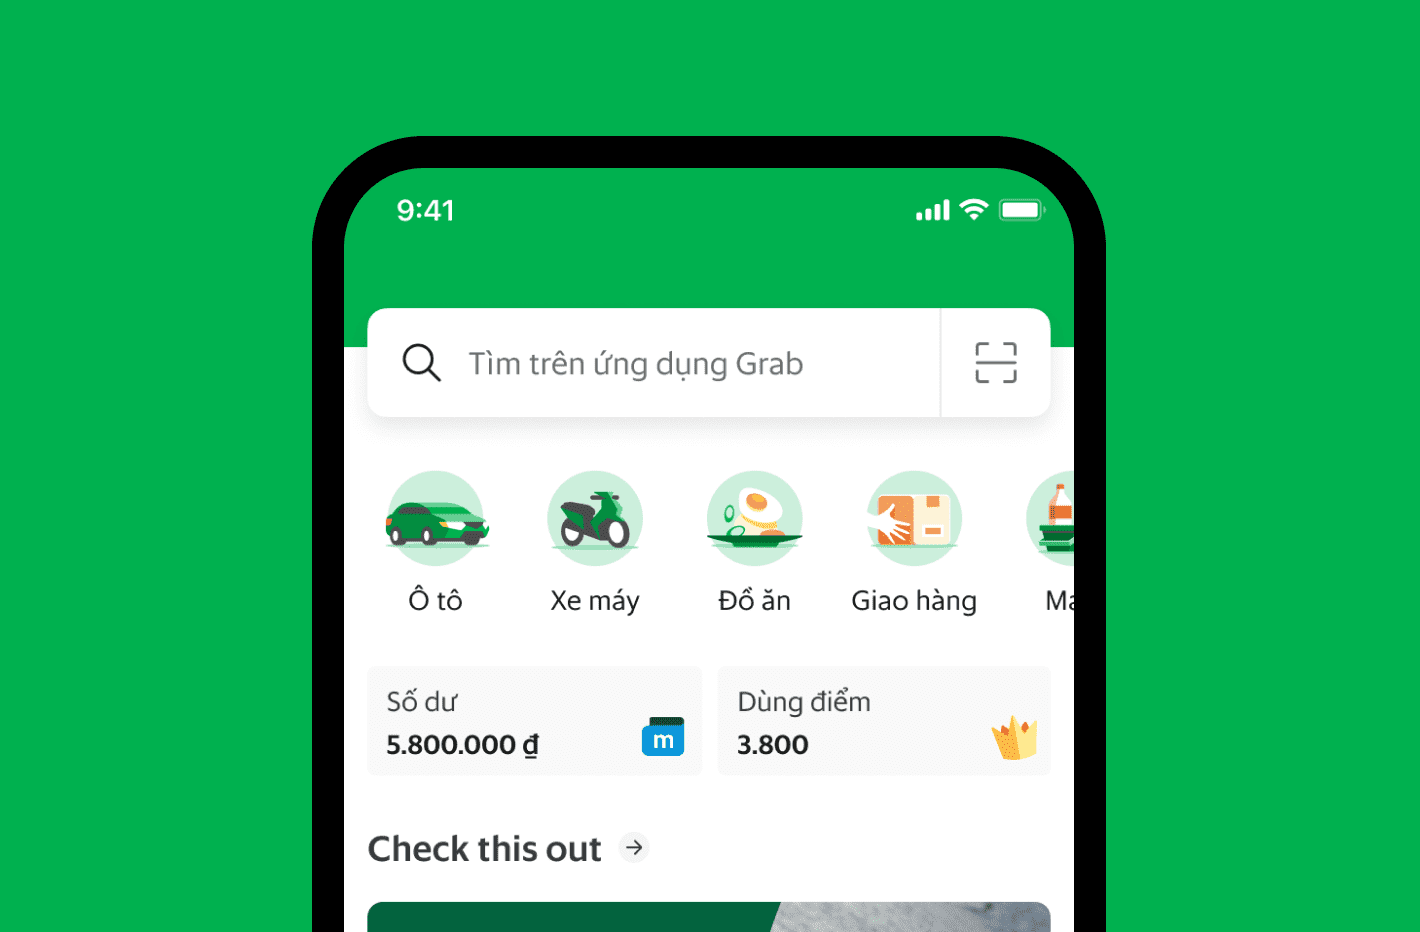
\includegraphics[width=\textwidth]{grab1.png}
    \end{minipage}
    \hfill
    \begin{minipage}[b]{0.32\textwidth}
        \centering
        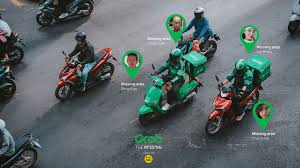
\includegraphics[width=\textwidth]{grab2.jpg}
    \end{minipage}
    \hfill
    \begin{minipage}[b]{0.32\textwidth}
        \centering
        
\includegraphics[width=\textwidth]{grab3.jpg}
    \end{minipage}
    \caption{Grab Rentals Interface}
    \label{fig:grab_interface}
\end{figure}

Grab Rentals is a transportation service platform embedded within the broader Grab super-app ecosystem, enabling users to book vehicles through a unified mobile interface. The platform prioritizes frictionless transactions and rapid booking confirmation within an established consumer base.

\begin{itemize}
    \item \textbf{Strengths:} Streamlined booking workflow with minimal user steps; tightly integrated online payment system; real-time booking confirmation and push notifications; extensive brand trust and large existing user base; strong mobile-first experience optimized for Southeast Asian markets.

    \item \textbf{Weaknesses:} Rigid rental duration options with limited customization; vehicle specification detail is often insufficient for informed decision-making; review and dispute transparency is constrained by the platform's black-box design; heavy dependency on the mobile application with no equivalent web interface; pricing complexity increases significantly during peak demand periods.

    \item \textbf{Analysis:} Grab Rentals delivers a highly efficient transactional experience optimized for speed and convenience. However, the platform is architecturally designed around Grab's B2C transportation model rather than a P2P asset-sharing paradigm. As a result, mechanisms for owner-renter communication, vehicle trust evaluation, and flexible listing customization are notably underdeveloped compared to dedicated rental marketplace standards.
\end{itemize}

\subsubsection{Traveloka Car Rental}

\begin{figure}[htbp]
    \centering
    \begin{minipage}[b]{0.45\textwidth}
        \centering
        
\includegraphics[width=\textwidth]{tv1.jpg}
    \end{minipage}
    \hfill
    \begin{minipage}[b]{0.45\textwidth}
        \centering
        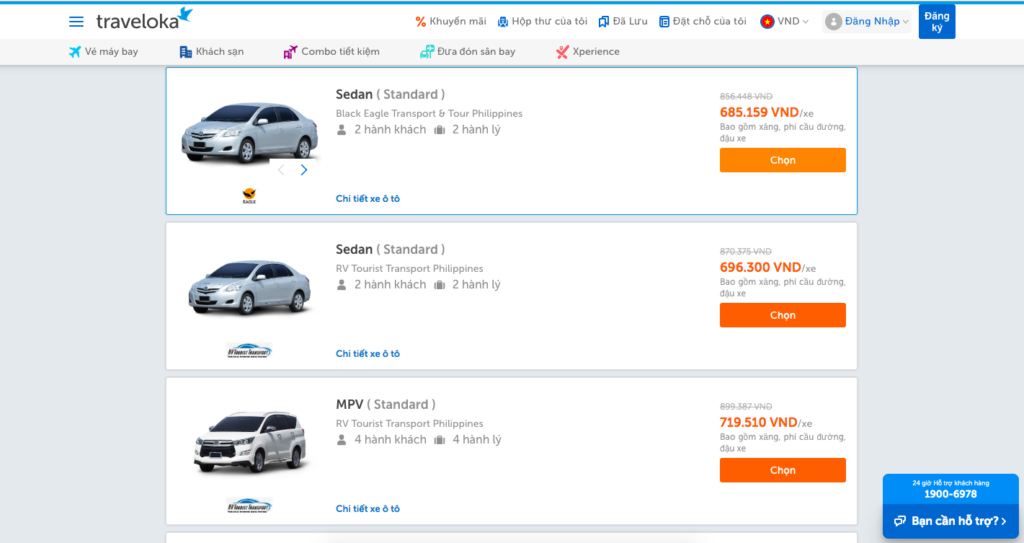
\includegraphics[width=\textwidth]{tv2.png}
    \end{minipage}
    \caption{Traveloka Car Rental Interface}
    \label{fig:traveloka_interface}
\end{figure}

Traveloka Car Rental is a vertical within the Traveloka travel super-platform, offering vehicle rental services tightly bundled with flight, hotel, and tourism booking capabilities. The service targets travelers seeking integrated itinerary management rather than standalone vehicle rental.

\begin{itemize}
    \item \textbf{Strengths:} Deeply integrated travel booking ecosystem enabling bundle pricing; diverse vehicle category coverage across major Vietnamese cities; reliable payment processing with consumer protection guarantees; established brand reputation across Southeast Asia; multi-criteria search and filtering tools.

    \item \textbf{Weaknesses:} Interface complexity increases cognitive load for users seeking a standalone rental experience; no direct messaging channel between renter and vehicle provider; a subset of bookings requires manual back-office confirmation, introducing operational latency; identity and review verification mechanisms are opaque to consumers.

    \item \textbf{Analysis:} Traveloka's rental vertical succeeds as a convenience layer for travelers already embedded in its ecosystem, but falls short as a dedicated P2P rental marketplace. The absence of direct owner-renter communication and the opacity of the review verification process represent material gaps relative to a trust-first rental platform such as LuxeWay.
\end{itemize}

\subsubsection{Local Vehicle Rental Websites}

\begin{figure}[htbp]
    \centering
    \begin{minipage}[b]{0.45\textwidth}
        \centering
        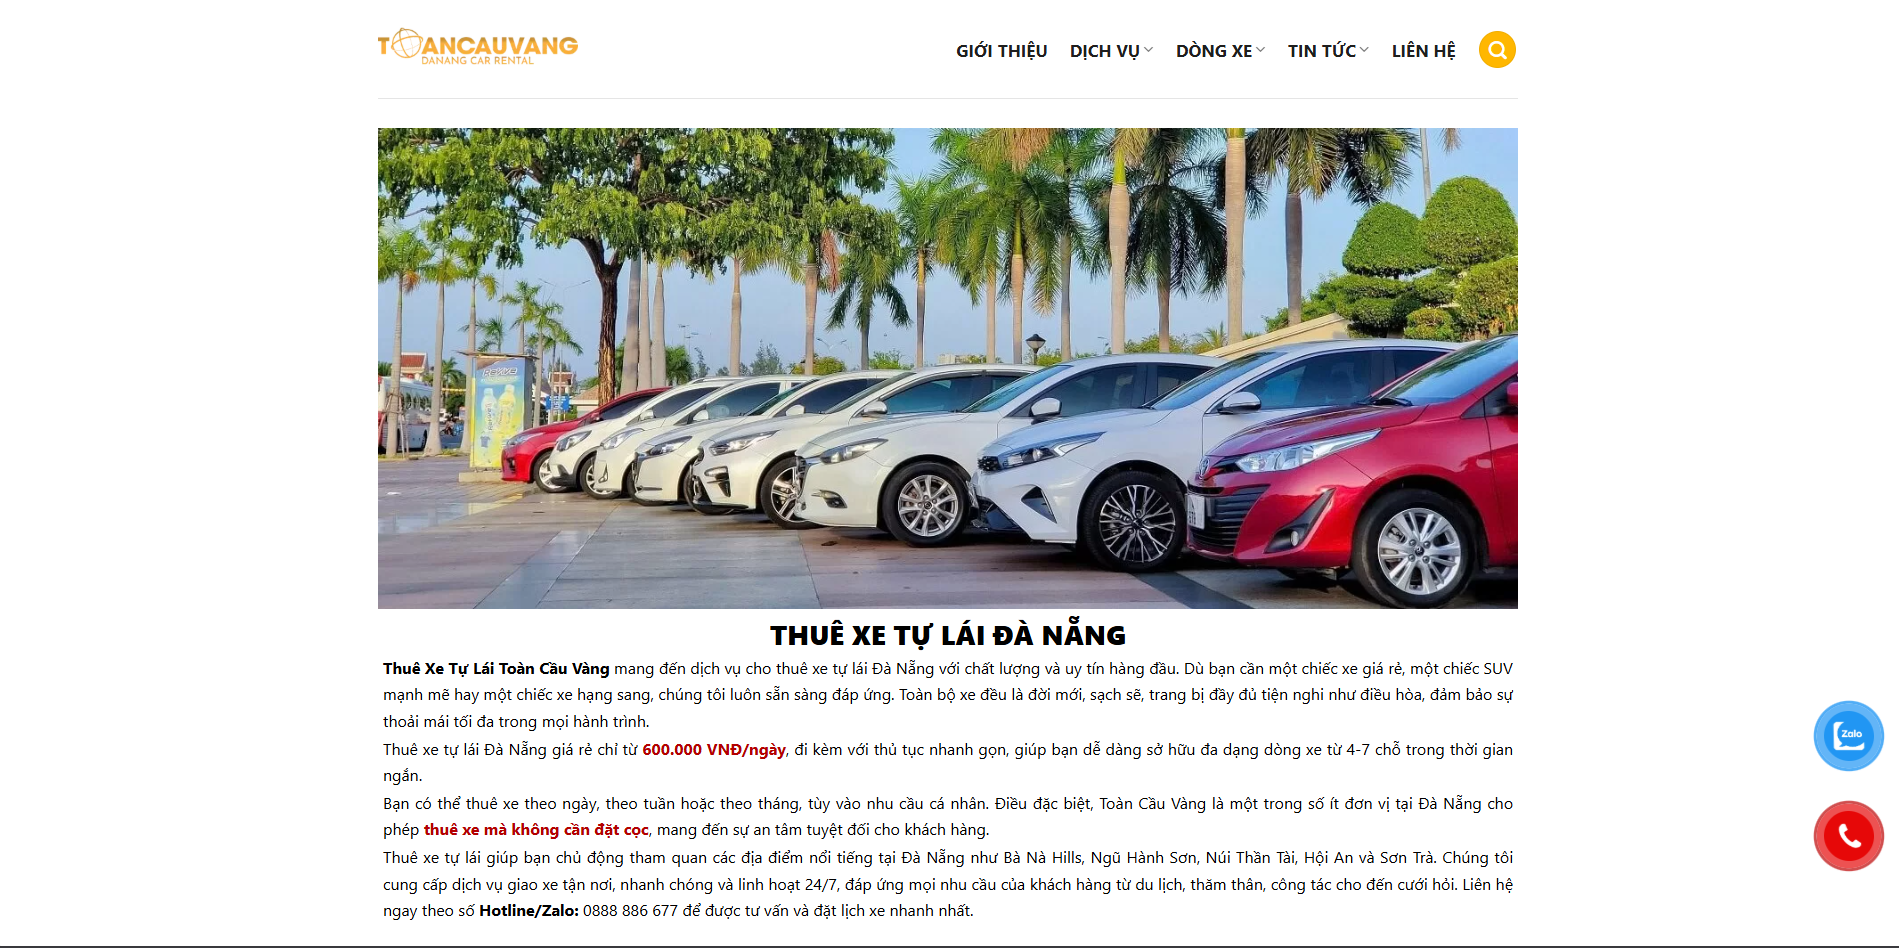
\includegraphics[width=\textwidth]{lcr1.png}
    \end{minipage}
    \hfill
    \begin{minipage}[b]{0.45\textwidth}
        \centering
        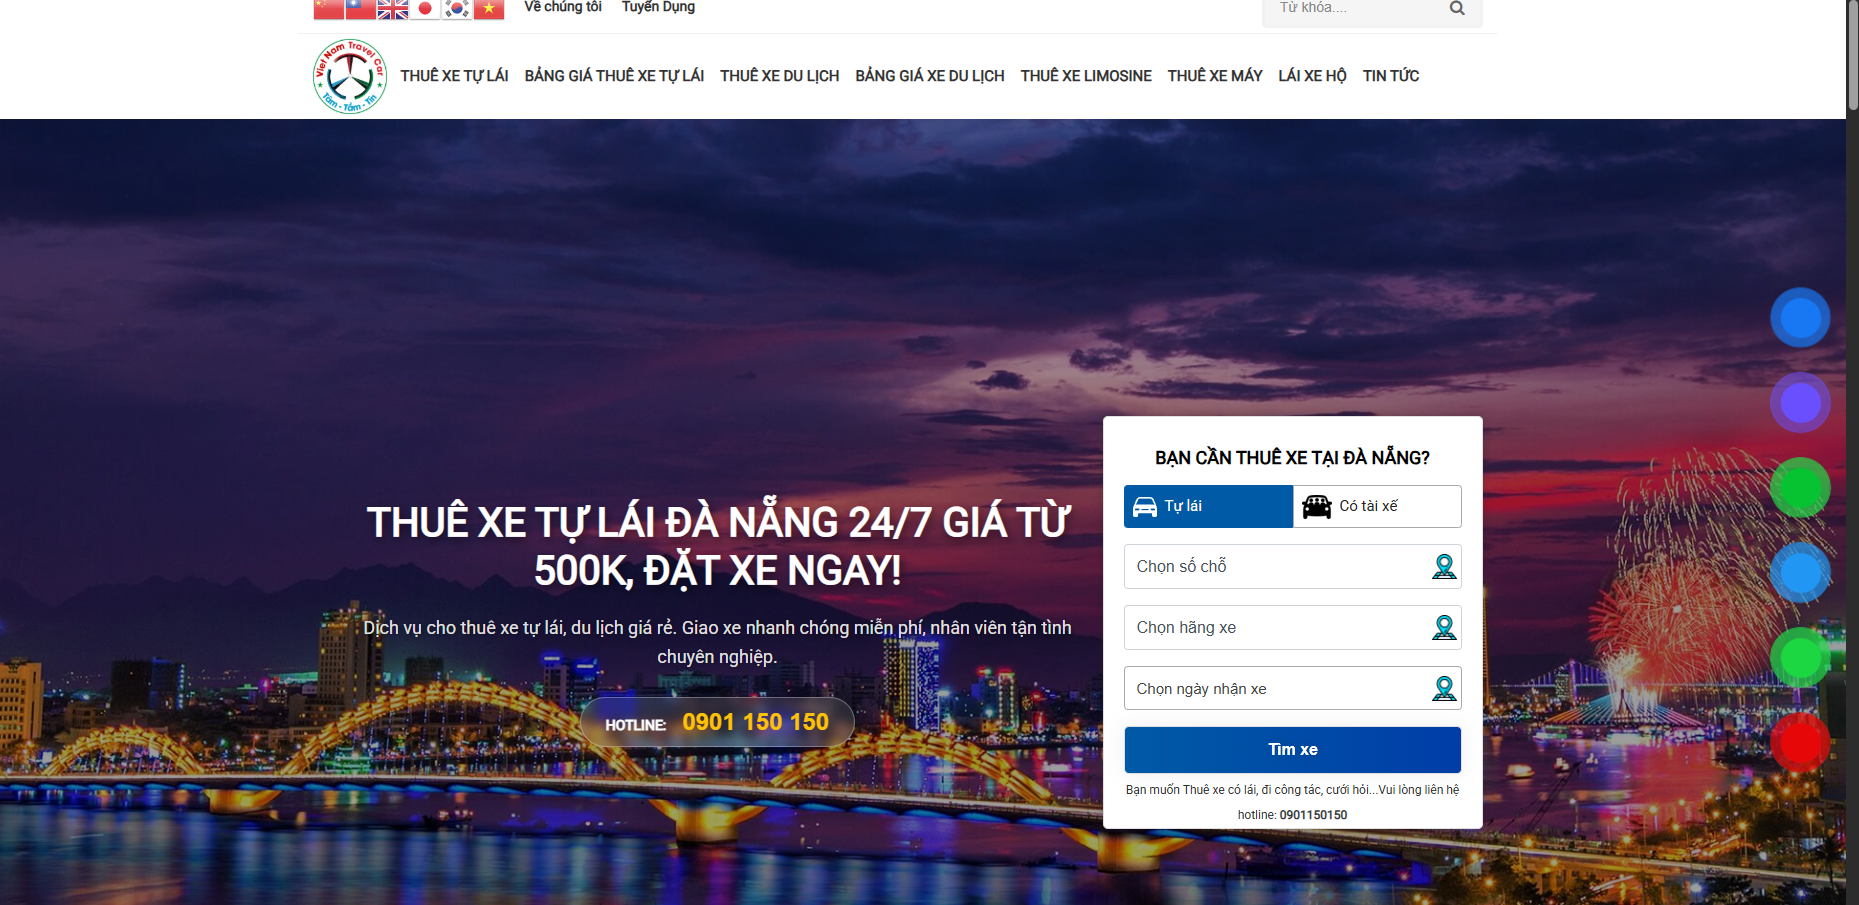
\includegraphics[width=\textwidth]{lcr2.png}
    \end{minipage}
    \caption{Local Vehicle Rental Website Examples}
    \label{fig:local_rental}
\end{figure}

Independent local rental operators in Vietnam typically maintain bespoke booking websites with varying levels of technical sophistication. These systems generally provide basic vehicle listing, contact-based booking requests, and manual payment confirmation.

\begin{itemize}
    \item \textbf{Strengths:} Flexible pricing and negotiation; personalized customer support; simpler booking workflows suited to repeat customers.

    \item \textbf{Weaknesses:} Weak authentication and security mechanisms; outdated and non-responsive UI/UX design; limited payment gateway integration; absence of digital contract or booking audit trail; no verified review infrastructure; poor scalability beyond a single operator.

    \item \textbf{Analysis:} While local rental websites offer flexibility and direct owner interaction, they consistently lack the standardized security practices, scalable booking workflows, digital contract support, and trust infrastructure required for a credible P2P marketplace. Their fragmented nature creates an unmet market need for a consolidated, trustworthy rental platform.
\end{itemize}

\subsection{Comparative Summary}

\begin{table*}[ht]
\centering
\caption{Comparative Summary of Existing Rental Systems}
\label{tab:existing_systems}
\begin{tabular}{p{3.2cm} p{6cm} p{6cm}}
\toprule
\textbf{System} & \textbf{Key Strengths} & \textbf{Key Weaknesses} \\
\midrule
Grab Rentals & Fast booking; large user base; integrated payments & No web interface; rigid options; limited trust transparency \\
Traveloka Car Rental & Broad vehicle range; trusted brand; bundle pricing & No owner-renter chat; opaque reviews; manual confirmation \\
Local Rental Websites & Flexible pricing; personalized service & Weak security; no digital contracts; no verified reviews \\
\bottomrule
\end{tabular}
\end{table*}

\subsection{Implications for LuxeWay}

The analysis of existing platforms reveals a consistent set of structural limitations that LuxeWay is specifically designed to address:

\begin{itemize}
    \item \textbf{Owner-renter communication gap} $\rightarrow$ WebSocket real-time chat (STOMP/SockJS)
    \item \textbf{Single-dimension or opaque ratings} $\rightarrow$ Five-dimension review model per verified booking
    \item \textbf{No direct P2P listing control} $\rightarrow$ Owner self-service listing with full specification, image, and pricing management
    \item \textbf{Limited payment localization} $\rightarrow$ VNPay gateway + LuxeWallet with Vietnamese bank and e-wallet support
    \item \textbf{No digital rental contracts} $\rightarrow$ Auto-generated PDF contract (iText) on booking confirmation
    \item \textbf{Manual or absent KYC} $\rightarrow$ Structured document upload and admin-driven verification workflow
    \item \textbf{Poor mobile-web consistency} $\rightarrow$ Responsive React SPA optimized for both desktop and mobile browsers
\end{itemize}

\section{Literature Review}

\subsection{Vehicle Rental Systems}

Traditional vehicle rental systems have long been characterized by manual booking processes, in-person identity verification, and centralized fleet management, each of which introduces operational inefficiencies and heightened susceptibility to fraud \cite{gupta2025double}. The academic response to these limitations has evolved along two principal trajectories. The first advocates for the digitization of identity verification workflows through KYC automation and document authentication pipelines, substantially reducing the overhead of manual screening while improving fraud detection accuracy. The second trajectory proposes the use of blockchain technology and Smart Contracts to establish immutable, self-executing rental agreements that eliminate reliance on centralized intermediaries \cite{madhusudan2019applying}. Protocols such as SePCAR further extend this framework by introducing Multi-Party Computation (MPC) for the generation of tamper-resistant access tokens, enabling secure vehicle handover even in offline conditions. While LuxeWay does not implement blockchain in its current version, these principles directly inform its emphasis on structured digital contracts, automated deposit handling, and transparent booking audit trails.

\subsection{Authentication and Security}

The security architecture of modern vehicle rental platforms is a well-established area of academic inquiry, driven by the growing volume of online transactions and the sensitivity of identity data exchanged during the rental lifecycle. Centralized authentication schemes are demonstrably vulnerable to credential stuffing, session hijacking, and unauthorized data access \cite{gupta2025double}. In response, the literature consistently advocates for stateless token-based authentication --- most commonly implemented via JSON Web Tokens (JWT) --- coupled with fine-grained role-based access control (RBAC) to constrain API surface exposure per user tier. LuxeWay operationalizes these recommendations directly: the backend enforces stateless JWT sessions with a 24-hour access token and a 7-day refresh token, while Spring Security's \texttt{HttpSecurity} configuration applies RBAC at the request-matcher level across four user roles (CUSTOMER, OWNER, ADMIN, SUPER\_ADMIN). OAuth2 social authentication via Google is additionally supported, with automatic email-based account linking to reduce onboarding friction without sacrificing identity assurance.

\subsection{Payment Systems}

The evolution of payment infrastructure in P2P rental platforms reflects a broader transition from cash-on-delivery and manual bank transfer to real-time, gateway-intermediated digital payments. In decentralized architectures, cryptocurrencies such as Ether enable direct peer-to-peer settlement, theoretically eliminating commission intermediaries entirely \cite{elhog2025decentralized}. Smart Contract escrow mechanisms further automate deposit release conditional on the fulfillment of predefined rental terms --- including on-time vehicle return and condition thresholds --- thereby reducing the need for manual dispute arbitration \cite{madhusudan2019applying}. LuxeWay adapts the escrow-and-release principle to the Vietnamese regulatory context by integrating \textbf{VNPay}'s payment gateway, which supports the full spectrum of domestic payment instruments (bank cards, MoMo, ZaloPay) alongside international Visa and Mastercard processing. The \textbf{LuxeWallet} internal balance further enables instant inter-party settlement without gateway round-trips. The pricing engine dynamically computes total booking cost across base rental, insurance tier selection, delivery fees, service charges, taxes, and coupon discounts, ensuring full pricing transparency prior to payment confirmation.

\subsection{Review and Rating Systems}

Reputation systems constitute the foundational trust layer of sharing-economy platforms, directly influencing booking conversion rates and platform retention \cite{hu2019sharing}. The inherent weakness of voluntary, text-based review systems --- susceptibility to fake reviews, reciprocal rating inflation, and selection bias among reviewers --- has been extensively documented in the literature. Proposed remedies range from algorithmic anomaly detection on review corpora to the integration of objective telematics signals sourced directly from vehicle OBD-II ports \cite{neifer2024trust}. Telematics-augmented reputation systems can evaluate driver behavior (speed compliance, braking patterns, mileage accuracy) independently of subjective reviewer opinion, substantially raising the bar for review manipulation. LuxeWay incorporates the conceptual insight of multi-signal trust evaluation by decomposing the post-rental review into five independently scored dimensions: vehicle cleanliness, listing accuracy, owner communication responsiveness, value for money, and delivery quality. Composite scores are aggregated and exposed on both vehicle listing pages and owner profiles, enabling prospective renters to make informed decisions grounded in a richer signal than a single aggregate star rating.

\section{Comparative Analysis of Related Research}

\subsection{Comparative Table of Related Research Studies}

Table~\ref{tab:lit_matrix} synthesizes the core literature evaluated
during the LuxeWay design phase, mapping each work's contribution,
limitations, and specific relevance to architectural and business
decisions embedded in the platform.

% table* spans both columns in IEEEtran two-column layout
\begin{table*}[ht]
\centering
\caption{Comparative Matrix of Related Work}
\label{tab:lit_matrix}
\begin{tabular}{p{2.2cm} p{3.8cm} p{3cm} p{3cm} p{3.5cm}}
\toprule
\textbf{Research Paper} &
\textbf{Main Contribution} &
\textbf{Strengths} &
\textbf{Limitations} &
\textbf{Relation to LuxeWay} \\
\midrule
Gupta et al.\ \cite{gupta2025double} &
Modern vehicle rental platform using MERN stack. &
Structured UI/UX workflows and admin dashboards. &
Centralized MongoDB creates single points of failure. &
Foundational reference for RESTful API and role-based UI design. \\
\midrule
Madhusudan \cite{madhusudan2019applying} &
Decentralized booking/payment on Ethereum with ECIES encryption. &
High-integrity transactions and automated penalties. &
Prohibitive gas fees and confirmation latency. &
Informs escrow-based deposit logic and digital contract design. \\
\midrule
El~Hog et al.\ \cite{elhog2025decentralized} &
Hybrid CarChain architecture (BSC + Firebase). &
Optimized throughput and reduced intermediary costs. &
Residual dependency on centralized storage. &
Paradigm for minimizing transaction overhead. \\
\midrule
Soppert et al.\ \cite{soppert2024benefit} &
Economic optimization model unifying CR and CS fleet usage. &
Quantified 23\%--120\% revenue increase from hybrid models. &
Scoped to B2C fleets; P2P legal dimensions unaddressed. &
Validates the CR+CS hybrid listing strategy in LuxeWay. \\
\midrule
Neifer et al.\ \cite{neifer2024trust} &
OBD telematics-driven reputation scoring for P2P rentals. &
Objective, manipulation-resistant trust signals. &
Requires physical OBD hardware per vehicle. &
Conceptual basis for LuxeWay's multi-dimensional review model. \\
\midrule
Kauffman \& Naldi \cite{kauffman2020research} &
Regulatory and economic landscape of sharing mobility. &
Systematic mapping of sustainable growth boundaries. &
Theoretical; no concrete system design. &
Informs platform compliance posture and market positioning. \\
\bottomrule
\end{tabular}
\end{table*}

\subsection{Synthesis and Design Implications}

Three cross-cutting observations emerge from this analysis and directly
shape LuxeWay's design:

\textbf{Technology.} The contrast between blockchain-native
solutions~\cite{madhusudan2019applying, elhog2025decentralized} and
conventional web stacks~\cite{gupta2025double} reveals a trade-off
between decentralization integrity and deployment pragmatism. LuxeWay
adopts a conventional full-stack architecture (React~18 + Spring
Boot~3 + SQL Server) while incorporating the \textit{behavioral
principles} of blockchain design---immutable records, transparent audit
trails, automated contracts---without on-chain execution overhead.

\textbf{Business model.} Soppert et al.'s~\cite{soppert2024benefit}
finding that hybrid CR+CS fleet management yields 23--120\% revenue
improvement justifies LuxeWay's dual-ecosystem architecture supporting
both daily car rental and shorter-duration motorbike sharing under one
owner dashboard.

\textbf{Trust infrastructure.} The spectrum from subjective reviews to
telematics-driven scoring~\cite{neifer2024trust} identifies a practical
middle ground: a structured multi-dimensional review protocol that
increases signal richness without requiring per-vehicle hardware,
preserving accessibility for individual private owners.

\section{Research Gaps}

\subsection{Insufficient Practical Implementation of Secure P2P Rental Platforms}

While the body of academic literature on P2P vehicle sharing is substantial, it disproportionately favors theoretical models and prototype demonstrations over production-grade, deployable implementations. Systems such as eKar and Sharik, while cited as market examples, remain highly centralized in their trust and payment architectures, replicating the intermediary dependency they ostensibly seek to eliminate. There is a notable absence of rigorously documented full-stack implementations that address the practical engineering challenges of session security, payment localization, real-time communication, and dispute management in a coherent, integrated system. LuxeWay contributes to closing this gap by providing a fully deployed web platform with documented architectural decisions.

\subsection{Underexplored Hybrid CR+CS Models in the P2P Context}

The combined Car Rental and Car Sharing model has been explored primarily within B2C commercial fleet optimization contexts \cite{soppert2024benefit}. Its application to platforms where individual private owners act as supply-side participants introduces qualitatively different challenges: irregular vehicle availability, heterogeneous asset quality, variable owner responsiveness, and the absence of centralized fleet maintenance standards. These P2P-specific dynamics remain insufficiently modeled in the optimization literature, representing a significant gap between theoretical fleet economics and the operational realities of consumer-grade P2P marketplaces.

\subsection{Absence of UX-Centered System Design Documentation}

The engineering literature on vehicle rental platforms --- particularly within the blockchain and decentralized systems tradition --- demonstrates a persistent bias toward back-end security architecture at the expense of front-end usability and interaction design. Specific deficiencies include:

\begin{itemize}
    \item Incomplete documentation of UI component architecture and client-side state management strategies.
    \item Absence of accessibility compliance analysis for rental booking flows.
    \item Insufficient treatment of multi-language localization in markets such as Vietnam, where bilingual (Vietnamese/English) interfaces are commercially necessary.
    \item Minimal attention to responsive design across device form factors, despite the dominance of mobile browsing in Southeast Asian markets.
    \item Heavy dependence on theoretical models and simulations without large-scale real-world testing.
\end{itemize}

LuxeWay addresses these gaps by adopting a component-driven frontend architecture (React 18 + Radix UI + Tailwind CSS) with explicit internationalization support (i18next) and accessibility-first design patterns.

\subsection{Limitations of Subjective-Only Reputation Systems}

Voluntary review mechanisms remain the dominant trust-signaling instrument across existing platforms, despite well-documented vulnerabilities to fake review injection, rating reciprocity bias, and score convergence toward inflated means \cite{hu2019sharing}. The telematics-based approach proposed by Neifer et al.\ \cite{neifer2024trust} provides a compelling alternative but demands per-vehicle hardware investment that is impractical for casual private owners. The intermediate design space --- structured review decomposition, verified booking linkage, and temporal review analysis --- remains underexplored and represents an actionable research direction with immediate applicability to consumer P2P platforms.

\subsection{Unresolved Legal and Insurance Dimensions of P2P Rental}

The legal architecture supporting P2P vehicle sharing in Vietnam remains underdeveloped relative to mature markets such as the United States and the European Union. Key unresolved questions include the insurance liability boundary between personal vehicle policies and commercial rental usage, regulatory classification of P2P rental income, and the evidentiary weight of digitally generated rental contracts in dispute adjudication. Future iterations of LuxeWay must engage with these dimensions not merely as compliance requirements but as product design constraints that affect deposit structures, cancellation policies, and the scope of the platform's dispute resolution guarantee.

\section{Proposed Solution}

\subsection{Overview}

LuxeWay is implemented as a production-grade full-stack web application
organized into two independently deployable service boundaries: a
\textbf{React Single-Page Application (SPA)} serving the consumer and
owner interfaces, and a \textbf{Spring Boot RESTful API} encapsulating
all business logic, data persistence, and external service integration.

Although blockchain and Smart Contract capabilities identified in the
literature remain outside the current implementation scope, the
\textit{design principles} they embody---transactional atomicity, audit
immutability, automated condition enforcement, and privacy-preserving
identity management---are realized through analogous mechanisms within
the conventional stack: database transactions with optimistic locking,
append-only booking history tables, rule-based pricing automation, and
JWT-scoped data access.

\subsection{System Architecture}

\subsubsection{Frontend}

The client application is built on \textbf{React~18} with
\textbf{TypeScript}, bundled by \textbf{Vite~5}, and styled with
\textbf{Tailwind CSS~3} and \textbf{Radix UI} accessible component
primitives. State is managed globally via \textbf{Zustand} stores for
authentication, vehicle browsing, and wishlist. Additional libraries
include React Router~6.25 (routing), Framer Motion~11.3 (animation),
React Leaflet~4.2 (map display), i18next~26.2 (Vi/En i18n),
SockJS+STOMP (WebSocket messaging), React Hook Form + Zod~3.23 (form
validation), and Recharts~2.12 (dashboard visualization).

\subsubsection{Backend}

The server-side application is built on \textbf{Spring Boot~3.2.5}
running on \textbf{Java~21~LTS}, exposing a stateless RESTful API at
context path \texttt{/api/v1}. Table~\ref{tab:backend_stack} summarizes
the principal backend components.

\begin{table}[htbp]
\centering
\caption{Backend Technology Stack}
\label{tab:backend_stack}
\begin{tabular}{ll}
\toprule
\textbf{Technology} & \textbf{Purpose} \\
\midrule
Spring Boot 3.2.5 / Java 21  & REST API, embedded Tomcat \\
Spring Data JPA + Hibernate 6 & ORM, JPQL queries \\
Spring Security + JJWT 0.12.3 & JWT auth, RBAC, OAuth2 \\
Spring WebSocket + STOMP      & Real-time messaging \\
SpringDoc OpenAPI 2.5         & Swagger UI documentation \\
MapStruct 1.5                 & Entity-to-DTO mapping \\
iText 5.5                     & PDF contract generation \\
Apache Tika 2.9               & File upload MIME validation \\
Lombok 1.18                   & Boilerplate code generation \\
\bottomrule
\end{tabular}
\end{table}

\subsubsection{Database}

\textbf{Microsoft SQL Server} serves as the primary relational data
store, managed through Hibernate schema validation (\texttt{ddl-auto:
none}) with explicit SQL schema scripts. The schema comprises over~40
tables organized into nine logical domains: Identity \& Access; Vehicle
Ecosystem (Cars); Vehicle Ecosystem (Motorbikes); Booking Lifecycle;
Payments; Trust \& Reviews; Communication; Support \& Knowledge; and
Platform Analytics. Schema initialization and seed data are applied
automatically on startup via Spring's \texttt{sql.init} subsystem.

\subsubsection{API Design}

The backend exposes a versioned RESTful API following standard HTTP
semantics. Principal endpoint groups include: \texttt{/auth/**}
(registration, login, token refresh, OAuth2); \texttt{/cars/**} and
\texttt{/motorbikes/**} (listing, search, booking); \texttt{/payments/**}
(VNPay checkout and callback); \texttt{/reviews/**} (post-rental
submission); \texttt{/users/**} (profile, KYC upload); and
\texttt{/admin/**} (ADMIN/SUPER\_ADMIN only). CORS is configured
globally to permit \texttt{localhost:5173} and production frontend
origins with \texttt{AllowCredentials: true}.

\subsection{Strategic Business Model}

LuxeWay operationalizes the hybrid CR+CS model validated by Soppert
et al.~\cite{soppert2024benefit} by maintaining two structurally
independent vehicle ecosystems---\textbf{Cars} and
\textbf{Motorbikes}---under a unified owner dashboard. This architecture
is hypothesized to increase per-owner revenue in the 23--120\% range
documented for commercial fleet operators~\cite{soppert2024benefit},
adapted to the P2P context where individuals constitute the supply side.

A transparent fee structure applies at checkout: a 12\% service fee
and 8\% tax on the base rental price, consistent with Vietnamese
e-commerce norms. Insurance tiers (basic, premium, zero-deductible),
delivery fees, add-on packages (chauffeur, airport delivery, wedding),
and coupon codes are composited into the final booking total prior to
VNPay initiation.

\subsection{Security Architecture}

\subsubsection{Authentication and Session Management}

LuxeWay implements stateless JWT authentication (RFC~7519). Login
issues a signed access token (24\,h expiry) and refresh token (7\,d
expiry) via HS256. The frontend client intercepts 401 responses,
silently refreshes the token, and retries the original request.
OAuth2 via Google is supported; the backend links the OAuth2 identity
to an existing account by email or creates a new one, then issues an
equivalent JWT pair.

\subsubsection{Role-Based Access Control}

Authorization is enforced at two layers. \texttt{HttpSecurity}
\texttt{requestMatchers} rules restrict paths by HTTP method and
role---e.g., \texttt{GET /cars/**} is public while \texttt{POST /cars}
requires \texttt{OWNER} or \texttt{ADMIN}. Service-layer
\texttt{@PreAuthorize} annotations enforce ownership constraints at
the business logic level.

\subsubsection{Payment and File Security}

A custom \texttt{VNPayIPWhitelistFilter} validates that VNPay callbacks
originate exclusively from declared VNPay server IPs, preventing spoofed
callback injection. Uploaded files are validated by Apache Tika's
MIME-type detector against declared \texttt{Content-Type}, mitigating
polyglot file upload attacks.

\subsection{Multi-Dimensional Review System}

Following the framework of Neifer et al.~\cite{neifer2024trust},
LuxeWay replaces a single-axis star rating with a five-dimension model
applied per verified completed booking (Table~\ref{tab:review_dims}).
Each dimension is scored 1--5; the composite rating is the arithmetic
mean. Mandatory booking linkage eliminates unverified submissions,
reducing the manipulation risk documented in~\cite{hu2019sharing}.

\begin{table}[htbp]
\centering
\caption{Five-Dimension Review Model}
\label{tab:review_dims}
\begin{tabular}{ll}
\toprule
\textbf{Dimension} & \textbf{Evaluated Aspect} \\
\midrule
Vehicle Cleanliness  & Physical condition at pickup \\
Listing Accuracy     & Description vs.\ actual vehicle \\
Owner Communication  & Responsiveness and professionalism \\
Value for Money      & Quality-to-price ratio \\
Delivery Quality     & Timeliness of vehicle delivery \\
\bottomrule
\end{tabular}
\end{table}

\section{Conclusion}

This paper has presented the design rationale, architectural decisions, and implementation approach of \textbf{LuxeWay} --- a peer-to-peer vehicle rental marketplace developed for the Vietnamese market. Through a systematic analysis of incumbent platforms and a structured review of the academic literature, the work identified four persistent gaps in existing systems: the absence of production-grade P2P implementations, insufficient support for hybrid CR+CS business models in the P2P context, neglect of UX-centered system documentation, and the limitations of subjective-only reputation systems.

LuxeWay addresses each of these gaps through deliberate engineering choices. The full-stack architecture --- \textbf{React 18 + TypeScript} on the frontend and \textbf{Spring Boot 3 / Java 21} on the backend, backed by \textbf{Microsoft SQL Server} --- delivers a deployable, maintainable system that embodies the behavioral principles of secure, transparent P2P rental without incurring the operational complexity of blockchain deployment. The hybrid Car and Motorbike listing ecosystem validates Soppert et al.'s \cite{soppert2024benefit} revenue optimization thesis in a P2P context. The multi-dimensional review protocol adapts Neifer et al.'s \cite{neifer2024trust} objectivity argument to a hardware-free implementation accessible to individual owners. The VNPay + LuxeWallet payment infrastructure localizes the trust-and-escrow principles of Smart Contract payment systems \cite{madhusudan2019applying} to the Vietnamese regulatory and banking environment.

Findings from related studies confirm that platforms combining Car Rental and Car Sharing models can achieve significant economic benefits for both vehicle owners and consumers \cite{elhog2025decentralized, soppert2024benefit}. By grounding implementation decisions in the academic literature while remaining pragmatic about deployment constraints, LuxeWay demonstrates that a trustworthy, feature-complete P2P rental marketplace is achievable with conventional web technologies when architectural principles are applied with rigor.

Future work will explore the integration of AI-driven vehicle recommendation, native mobile application development, and --- as the Vietnamese regulatory landscape matures --- selective incorporation of smart contract escrow mechanisms for high-value rental transactions.


% --- References ---
\balance  % Balance the two columns on the final page
\bibliographystyle{IEEEtran}
\bibliography{references}

\end{document}
